\chapter{گرافلت کرنل گاوسی}\label{chap:gaussian-graphlet-kernel}
گرافلت‌ها انتخاب خوبی برای مقایسه دو گراف هستند. دلیل این انتخاب اولاً \خمیده{فرضیه بازسازی گراف}\پانوشت{\متن‌لاتین{graph reconstruction conjecture}}\جستار{Kelly_1957} است که بیان می‌کند هر گراف بطور یکتا توسط زیرگراف‌هایش مشخص می‌شود. بنابراین انتظار داریم اگر دو گراف شبیه هم باشند، گردایه‌ی زیرگراف‌های آن‌ها نیز مشابه باشد. ثانیاً به دلیل استفاده از تعداد زیرگراف‌های با اندازه ثابت، این مقایسه دچار مشکل رفت و برگشت و هالتینگ نمی‌شود.
در این فصل ابتدا نحوه شمارش گرافلت‌ها را شرح داده و سپس گرافلت کرنل گاوسی را معرفی می‌کنیم و به سنجش قدرت آن در جداسازی مدل‌های تصادفی گراف از یکدیگر، می‌پردازیم.

\section{گرافلت‌ها و شمارش آن‌ها}
گرافلت‌ها، زیرگراف‌های کوچک القایی بین سه تا پنج رأس از یک گراف بزرگتر هستند\جستار{Przulj_2004} که با برچسب $G1,\ldots,G29$ در شکل \ارجا{fig:graphlets} نمایش داده شده‌اند (معمولاً زیرگراف تک یالی $G0$ هم به این مجموعه اضافه می‌شود).  رئوس هر گرافلت به گروه‌های خودریختی\پانوشت{\متن‌لاتین{automorphism}} تقسیم می‌شوند که به آن‌ها اوربیت\پانوشت{\متن‌لاتین{orbit}} گفته می‌شود. دو رأس از یک گرافلت به یک گروه اوربیتی تعلق دارند اگر توسط یک تابع خودریختی به یکدیگر نگاشت شوند. در شکل \ارجا{fig:graphlets} اوربیت‌ها با اعداد صفر تا 72 روی هر گرافلت مشخص شده‌اند و رنگ رئوس نشان‌دهنده تعلق آن‌ها به یک گروه اوربیتی است. از گرافلت‌ها و اوربیت‌ها در اندازه‌گیری شباهت ساختاری شبکه‌های تعاملات پروتئینی\پانوشت{\متن‌لاتین{Protein Interaction Networks}}\جستار{Przulj_2007}، انتخاب مدل تصادفی برای آن‌ها\جستار{Przulj_2004} و همچنین برای تراز کردن\پانوشت{\متن‌لاتین{alignment}} این شبکه‌ها\جستار{Milenkovic_2010}\جستار{Kuchaiev_2010}\جستار{Memisevic_2012} استفاده شده‌است.

شمارش گرافلت‌های یک گراف (و طبیعتاً اوربیت‌ها) از لحاظ محاسباتی بسیار زمانبر است. به همین دلیل معمولاً از روش‌های نمونه‌برداری برای تخمین تعداد آن‌ها استفاده می‌شود\جستار{Rahman_2014}\جستار{Milenkovic_2008}. به تازگی الگوریتم ترکیبیاتی شمارش اوربیت‌ها\جستار{Hovcevar_2014} ارائه شده‌است که تعداد آن‌ها را به طور دقیق و در زمان بسیار کم محاسبه می‌نماید. با کمی تغییر در این الگوریتم، می‌توان بجای اوربیت‌ها، تعداد گرافلت‌ها را بدست آورد. ذکر این نکته ضروری است که برخلاف تصور، استفاده از اوربیت‌ها برای تعریف کرنل (بجای گرافلت‌ها) موجب افزایش نویز و در نتیجه، کاهش دقت می‌گردد. در بخش \ارجا{sec:graphlet-vs-orbit} به بررسی این مسئله می‌پردازیم.


\begin{figure}[t]
\center{
\begin{tikzpicture}[scale=1.5,transform shape]
% 2-node
    \node[node] (1) {};
    \node[node] (2) [below of=1] {};
    \path (1) edge (2);
    \node [below of=2] {\lr{G0}};
% 3-node
    \node[node] (3) [below right=-0.4 and 0.7 of 1] {};
    \node[node3] (4) [below of=3] {};
    \node[node] (5) [below of=4] {};
    \path (3) edge (4);
    \path (4) edge (5);
    \node [below of=5] {\lr{G1}};

    \node[node] (6) [right=0.5 of 3] {};
    \node[node] (7) [right=0.25 of 5] {};
    \node[node] (8) [right=0.35 of 7] {};
    \path (6) edge (7);
    \path (7) edge (8);
    \path (8) edge (6);
    \node [below right=0.1 and 0.12 of 7] {\lr{G2}};
% 4-node
    \node[node] (9) [below right=-0.4 and 0.9 of 6] {};
    \node[node3] (10) [below of=9] {};
    \node[node3] (11) [below of=10] {};
    \node[node] (12) [below of=11] {};
    \path (9) edge (10);
    \path (10) edge (11);
    \path (11) edge (12);
    \node [below of=12] {\lr{G3}};

    \node[node] (13) [right=0.5 of 10] {};
    \node[node3] (14) [below of=13] {};
    \node[node] (15) [right=0.25 of 12] {};
    \node[node] (16) [right=0.35 of 15] {};
    \path (13) edge (14);
    \path (14) edge (15);
    \path (14) edge (16);
    \node [below right=0.09 and 0.1 of 15] {\lr{G4}};

    \node[node] (17) [right=0.5 of 13] {};
    \node[node] (18) [right=0.35 of 17] {};
    \node[node] (19) at (16 -| 17) {};
    \node[node] (20) [right=0.35 of 19] {};
    \path (17) edge (18);
    \path (18) edge (20);
    \path (19) edge (20);
    \path (19) edge (17);
    \node [below right=0.09 and 0.1  of 19] {\lr{G5}};

    \node[node2] (21) [right=0.5 of 18] {};
    \node[node3] (22) [below of=21] {};
    \node[node] (23) [right=0.25 of 20] {};
    \node[node] (24) [right=0.35 of 23] {};
    \path (21) edge (22);
    \path (22) edge (23);
    \path (22) edge (24);
    \path (23) edge (24);
    \node [below right=0.09 and 0.1 of 23] {\lr{G6}};

    \node[node3] (25) [right=0.5 of 21] {};
    \node[node] (26) [right=0.35 of 25] {};
    \node[node] (27) at (24 -| 25) {};
    \node[node3] (28) [right=0.35 of 27] {};
    \path (25) edge (26);
    \path (26) edge (28);
    \path (27) edge (28);
    \path (25) edge (27);
    \path (25) edge (28);
    \node [below right=0.09 and 0.1 of 27] {\lr{G7}};

    \node[node] (29) [right=0.5 of 26] {};
    \node[node] (30) [below=0.20 of 29] {};
    \node[node] (31) [right=0.25 of 28] {};
    \node[node] (32) [right=0.35 of 31] {};
    \path (29) edge (30);
    \path (29) edge (31);
    \path (29) edge (32);
    \path (30) edge (31);
    \path (30) edge (32);
    \path (31) edge (32);
    \node [below right=0.09 and 0.1 of 31] {\lr{G8}};
\end{tikzpicture}%
\vspace{0.2cm}
\begin{tikzpicture}[scale=1.5,transform shape]
% 5-node
    \node[node] (1) {};
    \node[node3] (2) [below of=1] {};
    \node[node2] (3) [below of=2] {};
    \node[node3] (4) [below of=3] {};
    \node[node] (5) [below of=4] {};
    \path (1) edge (2);
    \path (2) edge (3);
    \path (3) edge (4);
    \path (4) edge (5);
    \node [below of=5] {\lr{G9}};

    \node[node4] (12) [right=0.40 of 2] {};
    \node[node2] (13) [below of=12] {};
    \node[node3] (14) [below of=13] {};
    \node[node] (15) [right=0.15 of 5] {};
    \node[node] (16) [right=0.35 of 15] {};
    \path (12) edge (13);
    \path (13) edge (14);
    \path (14) edge (15);
    \path (14) edge (16);
    \node [below right = 0.10 and 0.05 of 15] {\lr{G10}};

    \node[node] (17) [right=0.3 of 14] {};
    \node[node3] (18) [right of=17 ] {};
    \node[node] (19) [right of=18 ] {};
    \node[node] (20) [below of=18 ] {};
    \node[node] (21) [below=-0.47 of 18 ] {};
    \path (17) edge (18);
    \path (18) edge (19);
    \path (20) edge (18);
    \path (21) edge (18);
    \node [below of=20] {\lr{G11}};
    
    \node[node3] (22) [below right= -0.42 and 0.7 of 21] {};
    \node[node] (23) [below right=0.27 and -0.4 of 22] {};
    \node[node] (24) [below right=0.27 and 0.15 of 22] {};
    \node[node2] (25) [below=0.28 of 23] {};
    \node[node2] (26) [below=0.28 of 24] {};
    \path (22) edge (23);
    \path (22) edge (24);
    \path (23) edge (24);
    \path (23) edge (25);
    \path (24) edge (26);
    \node [below right= 0.10 and 0.05  of 25] {\lr{G12}};

    \node[node4] (27) [right=0.65 of 22] {};
    \node[node2] (28) [below of=27] {};
    \node[node3] (29) [below of=28] {};
    \node[node] (30) [right=0.1 of 26] {};
    \node[node] (31) [right=0.35 of 30] {};
    \path (27) edge (28);
    \path (28) edge (29);
    \path (29) edge (30);
    \path (29) edge (31);
    \path (30) edge (31);
    \node [below right = 0.10 and 0.05 of 30] {\lr{G13}};

    \node[node] (32) [right=0.35 of 28] {};
    \node[node] (33) [right=0.35 of 32] {};
    \node[node3] (34) [below right=0.15 and 0.15 of 32] {};
    \node[node2] (35) [right=0.1 of 31] {};
    \node[node2] (36) [right=0.35 of 35] {};
    \path (32) edge (34);
    \path (33) edge (34);
    \path (34) edge (35);
    \path (34) edge (36);
    \path (35) edge (36);
    \node [below right = 0.10 and 0.05 of 35] {\lr{G14}};

    \node[node] (37) [right=0.35 of 33] {};
    \node[node] (38) [below right=0.10 and -0.45 of 37] {};
    \node[node] (39) [right=0.5 of 38] {};
    \node[node] (40) [below right=0.20 and 0.03 of 38] {};
    \node[node] (41) [right=0.20 of 40] {};
    \path (37) edge (38);
    \path (37) edge (39);
    \path (39) edge (41);
    \path (38) edge (40);
    \path (41) edge (40);
    \node [below right = 0.10 and 0.02 of 40] {\lr{G15}};
    
    \node[node4] (42) [below right=-0.45 and 0.75 of 37] {};
    \node[node] (43) [below right=0.17 and -0.45 of 42] {};
    \node[node] (44) [right=0.45 of 43] {};
    \node[node3] (45) [below=0.4 of 42] {};
    \node[node2] (46) [below of=45] {};
    \path (42) edge (43);
    \path (43) edge (45);
    \path (42) edge (44);
    \path (44) edge (45);
    \path (45) edge (46);
    \node [below of=46] {\lr{G16}};

    \node[node4] (46) [right=0.7 of 42] {};
    \node[node] (47) [below right=0.17 and -0.45 of 46] {};
    \node[node] (48) [right=0.45 of 47] {};
    \node[node3] (49) [below=0.4 of 46] {};
    \node[node2] (50) [below of=49] {};
    \path (46) edge (47);
    \path (46) edge (48);
    \path (47) edge (49);
    \path (48) edge (49);
    \path (46) edge (49);
    \path (49) edge (50);
    \node [below of=50] {\lr{G17}};
    
    \node[node] (51) [right=0.07 of 48] {};
    \node[node] (52) [right=0.35 of 51] {};
    \node[node3] (53) [below right=0.15 and 0.15 of 51] {};
    \node[node] (54) [below right=0.15 and -0.40 of 53] {};
    \node[node] (55) [right=0.35 of 54] {};
    \path (51) edge (52);
    \path (51) edge (53);
    \path (52) edge (53);
    \path (53) edge (54);
    \path (53) edge (55);
    \path (55) edge (54);
    \node [below right = 0.10 and 0.05 of 54] {\lr{G18}};
    
    \node[node4] (56) [below right=-0.43 and 0.45 of 52] {};
    \node[node] (57) [below right=0.17 and -0.45 of 56] {};
    \node[node] (58) [right=0.45 of 57] {};
    \node[node3] (59) [below=0.4 of 56] {};
    \node[node2] (60) [below of=59] {};
    \path (56) edge (57);
    \path (56) edge (58);
    \path (57) edge (59);
    \path (58) edge (59);
    \path (59) edge (60);
    \path (57) edge (58);
    \node [below of=60] {\lr{G19}};
\end{tikzpicture}%
\vspace{0.2cm}
\begin{tikzpicture}[scale=1.5,transform shape,node distance=0.30cm,minimum size=0.17cm,inner sep=0,node/.style={circle,draw,fill,align=center}]

    \node[node3] [right=0.8 of 1] (6) {};
    \node[node] [below right=0.3 and -0.55 of 6] (7) {};
    \node[node] [below right=0.3 and 0.3 of 6] (8) {};
    \node[node3] [below=0.67 of 6] (9) {};
    \node[node] [below=0.27 of 6] (10) {};
    \path (6) edge (7);
    \path (6) edge (8);
    \path (7) edge (9);
    \path (8) edge (9);
    \path (6) edge (10);
    \path (10) edge (9);
    \node [below  of=9] {\lr{G20}};
    
    \node[node3] (11) [right=0.8 of 6] {};
    \node[node] (12) [below right=0.27 and -0.4 of 11] {};
    \node[node] (13) [below right=0.27 and 0.15 of 11] {};
    \node[node2] (14) [below=0.28 of 12] {};
    \node[node2] (15) [below=0.28 of 13] {};
    \path (11) edge (12);
    \path (11) edge (13);
    \path (12) edge (13);
    \path (13) edge (15);
    \path (12) edge (14);
    \path (15) edge (14);
    \node [below right= 0.12 and 0.05  of 14] {\lr{G21}};
    
    \node[node2] (16) [right=0.6 of 11] {};
    \node[node] (17) [below right=0.15 and -0.4 of 16] {};
    \node[node] (18) [right=0.36 of 17] {};
    \node[node2] (19) [below=0.36 of 16] {};
    \node[node2] (20) [below of=19] {};
    \path (16) edge (17);
    \path (16) edge (18);
    \path (17) edge (18);
    \path (17) edge (19);
    \path (18) edge (19);
    \path (17) edge (20);
    \path (18) edge (20);
    \node [below of=20] {\lr{G22}};
    
    \node[node] (23) [right=0.5 of 16] {};
    \node[node] (24) [below=0.18 of 23] {};
    \node[node3] (25) [below right=0.1 and -0.4 of 24] {};
    \node[node] (26) [right=0.35 of 25] {};
    \node[node2] (27) [below=0.1 of 25] {};
    \path (24) edge (23);
    \path (24) edge (25);
    \path (24) edge (26);
    \path (23) edge (25);
    \path (23) edge (26);
    \path (25) edge (26);
    \path (25) edge (27);
    \node [below right=0.12 and 0.07 of 27] {\lr{G23}};

    \node[node] (28) [right=0.3 of 23] {};
    \node[node3] (29) [below=0.25 of 28] {};
    \node[node] (30) [below=0.25 of 29] {};
    \node[node2] (31) [below right=0.11 and 0.2 of 28] {};
    \node[node2] (32) [below=0.2 of 31] {};
    \path (28) edge (29);
    \path (29) edge (30);
    \path (28) edge (31);
    \path (31) edge (32);
    \path (30) edge (32);
    \path (29) edge (31);
    \path (29) edge (32);
    \node [below right = 0.12 and 0.0 of 30] {\lr{G24}};
    
    \node[node] [right=0.8 of 28] (33) {};
    \node[node3] [below right=0.3 and -0.55 of 33] (34) {};
    \node[node2] [below right=0.3 and 0.3 of 33] (35) {};
    \node[node] [below=0.67 of 33] (36) {};
    \node[node3] [below=0.27 of 33] (37) {};
    \path (33) edge (34);
    \path (33) edge (35);
    \path (34) edge (36);
    \path (35) edge (36);
    \path (33) edge (37);
    \path (37) edge (36);
    \path (37) edge (34);
    \node [below  of=36] {\lr{G25}};
    
    \node[node3] (38) [right=0.7 of 33] {};
    \node[node] (39) [below right=0.15 and -0.4 of 38] {};
    \node[node] (40) [right=0.36 of 39] {};
    \node[node2] (41) [below=0.36 of 38] {};
    \node[node2] (42) [below of=41] {};
    \path (38) edge (39);
    \path (38) edge (40);
    \path (39) edge (40);
    \path (39) edge (41);
    \path (40) edge (41);
    \path (41) edge (42);
    \path (39) edge (42);
    \path (40) edge (42);
    \node [below of=42] {\lr{G26}};
    
    \node[node] (43) [right=0.8 of 38] {};
    \node[node] (44) [below right=0.3 and -0.55 of 43] {};
    \node[node] (45) [below right=0.3 and 0.3 of 43] {};
    \node[node] (46) [below=0.67 of 43] {};
    \node[node3] (47) [below=0.27 of 43] {};
    \path (43) edge (44);
    \path (43) edge (45);
    \path (44) edge (46);
    \path (45) edge (46);
    \path (43) edge (47);
    \path (47) edge (46);
    \path (47) edge (44);
    \path (47) edge (45);
    \node [below  of=46] {\lr{G27}};
    
    \node[node3] (48) [right=0.8 of 43] {};
    \node[node] (49) [below right=0.15 and -0.4 of 48] {};
    \node[node] (50) [right=0.36 of 49] {};
    \node[node] (51) [below=0.36 of 48] {};
    \node[node3] (52) [below of=51] {};
    \path (48) edge (51);
    \path (48) edge (49);
    \path (48) edge (50);
    \path (49) edge (50);
    \path (49) edge (51);
    \path (50) edge (51);
    \path (51) edge (52);
    \path (49) edge (52);
    \path (50) edge (52);
    \node [below of=52] {\lr{G28}};
    
    \node[node] (57) [right=0.4 of 50] {};
    \node[node] (58) [below right=0.10 and -0.45 of 57] {};
    \node[node] (59) [right=0.5 of 58] {};
    \node[node] (60) [below right=0.20 and 0.03 of 58] {};
    \node[node] (61) [right=0.20 of 60] {};
    \path (57) edge (58);
    \path (57) edge (59);
    \path (57) edge (60);
    \path (57) edge (61);
    \path (58) edge (59);
    \path (58) edge (60);
    \path (58) edge (61);
    \path (59) edge (61);
    \path (59) edge (60);
    \path (61) edge (60);
    \node [below right = 0.10 and 0.02 of 60] {\lr{G29}};
\end{tikzpicture}
}
\caption{گرافلت‌های دو تا پنج رأسی. رئوس همرنگ روی هر گرافلت، یک اوربیت را نمایش می‌دهند. شماره هر اوربیت روی یکی از رئوسش مشخص شده‌است.}
\label{fig:graphlets}
\end{figure}

\subsection{الگوریتم ترکیبیاتی شمارش گرافلت‌ها}
فرض کنید $x$ هر رأس از گراف $G$ باشد. مسئله، محاسبه تعداد دفعاتی است که $x$  روی اوربیت $O_i$ از گرافلت‌های القایی گراف $G$ قرار گرفته است. این عدد را با $o_i$ نمایش می‌دهیم. الگوریتم بر اساس دستگاهی از معادل خطی کار می‌کند که تعداد اوربیت‌های مختلف، $o_i$ ها، را به هم مربوط می‌کند. از آنجایی که رتبه این دستگاه یکی کمتر از تعداد انواع اوربیت‌ها خواهد بود می‌توان با شمارش تنها یکی از آن‌ها، تعداد مابقی را بدست آورد. در ادامه، نحوه ساخت و حل این دستگاه برای هر رأس را شرح داده و سپس روش محاسبه تعداد گرافلت‌های گراف از روی تعداد اوربیت رئوس را توضیح می‌دهیم.

\subsubsection{شمارش اوربیت‌های چهار رأسی}
%سمت راست معادلاتی که دستگاه را تشکیل می‌دهد شامل عباراتی است که از گراف $G$ محاسبه می‌شود.
فرض کنید $c(u,v) = |N(u) \cap N(v)|$ تعداد همسایه‌های مشترک دو رأس $u$ و $v$ باشد. همینطور $p(u,v)$ تعداد مسیرهای سه رأسی باشد که از رأس $u$ آغاز می‌شود، به رأس $v$ می‌رود و در رأسی مثل $t$ که به $u$ متصل نیست، پایان می‌یابد. این عدد به راحتی قابل محاسبه است: 
$p(u,v) = deg(v) -1 -c(u,v)$.

اگر رأس $x$ روی یک گرافلت $k$-رأسی مثل $G_i$ قرار گرفته باشد، حتماً روی یک گرافلت $(k-1)$-رأسی مثل $G_j$ هم قرار گرفته است، کافی است دورترین رأس از $x$ را از گراف $G_i$ حذف کنیم. زیرگرافی که از باقی رئوس بوجود می‌آید همبند است (در غیر این صورت، رأسی که جزء مؤلفه همبندی نیست دورترین رأس از $x$ بوده است) بنابراین با یکی از گرافلت‌های $(k-1)$-رأسی مثل $G_j$ یکریخت است.

عکس این مطلب نیز صحیح است: هر گرافلت چهار رأسی را می‌توان با افزودن یک رأس به یکی از گرافلت‌های سه رأسی ساخت. جهت یافتن رابطه تعداد اوربیت‌های گرافلت‌های چهار رأسی برای رأس $x$، تمام اوربیت‌های سه‌رأسی که $x$ روی آن‌ها قرار گرفته است را می‌یابیم و سپس امکان گسترش آن‌ها به گرافلت‌های چهار رأسی را بررسی می‌کنیم.

به عنوان مثال، همانطور که در شکل \ارجا{fig:o9-o12-relation} می‌بینید رئوس $x$،$y$ و $z$ گرافلت $G_1$ را القا می‌کنند که یک مسیر به طول دو است. این گرافلت، توسط $w$ و یال‌های $(w,y)$ و $(w,z)$ به یک گرافلت چهار رأسی تبدیل می‌شود. تعداد رأس‌های ممکن مثل $w$ برابر است با $c(y,z)$. در شکل $c(y,z) = 3$ تا از این رئوس وجود دارد که با $w_1$ ، $w_2$ و $w_3$ نشان داده شده‌اند. یال $(x,w)$ ممکن است در گراف $G$ وجود داشته باشد (مثلاً برای $w_3$ این حالت در نظر گرفته شده) یا ممکن است وجود نداشته باشد (رئوس $w_1$ و $w_2$ اینگونه‌اند). بدون این یال، رئوس $x$ ، $y$ ، $z$ و $w$ گرافلت $G_6$ را تشکیل می‌دهند که $x$ روی اوربیت $O_9$ قرار گرفته است. وجود این یال باعث می‌شود که رئوس مذکور، گرافلت $G_7$ را بسازند که در آن $x$ روی اوربیت $O_{12}$ قرار گرفته‌است. از آنجایی که تمام $c(y,z)$ رأس در $N(y) \cap N(z)$ باید یا در $G_7$ یا در $G_6$ باشند که متقابلاً باعث می‌شود $x$ در $O_9$ یا $O_{12}$ قرار گیرد، پس برای سه‌تایی $x$، $y$ و $z$ خواهیم داشت: $o_9 + o_{12} = c(y,z)$.

حال برای تمام مسیرهای به طول دو که از $x$ شروع می‌شوند، این عدد را جمع می‌زنیم. البته باید دقت داشت که در جمع، تقارن‌ها در نظر گرفته‌شوند: هر گرافلت $G_6$  در گراف $G$ ، با تعویض جای $z$ و $w$ دوبار شمره می‌شود. این اتفاق با تعویض $y$‌ و $w$ برای $G_7$ هم رخ می‌دهد. با این حساب می‌توانیم معادله زیر را تشکیل دهیم:
\begin{equation*}
2o_9+2o_{12} = \sum_{\substack{y,z: x,z\in N(y)\\G[\{x,y,z\}] \simeq G_1 }}c(y,z),
\end{equation*}
که در آن $G[\{x,y,z\}]$ زیرگراف القایی از $G$ است که توسط سه رأس $x$ ، $y$ و $z$ ساخته می‌شود.

برای مثالی دیگر، رابطه بین اوربیت‌های $O_6$ و $O_9$ را بررسی می‌کنیم. برای اینکار یک مسیر به طول دو از رئوس $x$ ، $y$ و $z$ را توسط یک مسیر دیگر که از $x$ و $y$ شروع می‌شود، گسترش می‌دهیم؛ قبلاً تعداد این مسیرها را با $p(x,y)$ نمادگذاری کردیم. بسته به اینکه رأس جدید ($w$) با $z$ همسایه باشد یا نه، با یک گرافلت $G_6$ یا $G_4$ روبرو هستیم. با احتساب تقارن، و همچنین حذف حالتی که در آن $w=z$ ، خواهیم داشت:
\begin{equation*}
2o_6+2o_9 = \sum_{\substack{y,z: x,z\in N(y)\\G[\{x,y,z\}] \simeq G_1 }}(p(x,y) - 1).
\end{equation*}

از آنجایی که تنها دو گرافلت سه رأسی وجود دارد و حالت‌های گسترش نیز محدود‌اند، می‌توان تمام گسترش‌های ممکن را در نظر گرفت و از آن‌ها یک دستگاه با ده معادله مستقل خطی و یازده متغیر (متناظر با یازده اوربیت گرافلت‌های چهار رأسی) استخراج کرد. در ضمیمه \ارجا{appendix:combinatorial-counting} این معادلات را آورده‌ایم.

عبارات موجود در سمت راست این معادلات، تنها وابسته به گراف $G$ هستند و باید برای هر رأس $x$ محاسبه شوند. برای افزایش سرعت اجرا، برای هر دو رأس $u$ و $v$ مقادیر $c(u,v)$ و $p(u,v)$ را از قبل محاسبه می‌کنیم. البته کافی است این مقادیر را تنها برای رئوس مجاور و نه همه رئوس، بدست آورد زیرا طبق تعریف، $p(u,v)$ فقط برای دو رأس مجاور تعریف می‌شود و همچنین در تمام معادلات به غیر از معادله آخر، $c(u,v)$ تنها برای رئوسی که همسایه هستند مورد نیاز است. بنابراین با اختصاص $O(m)$ فضا، این مقادیر را محاسبه می‌کنیم. برای معادله آخر، کافی است تعداد مسیر‌های به طول دو که از رأس $x$ شروع می‌شوند و به رأس $y$ خاتمه می‌یابند را بشماریم. این کار نیاز به $O(n)$ فضا دارد. چون تعداد اوربیت‌ها را برای هر رأس جداگانه شمارش می‌کنیم، می‌توان از این فضا مجدداً استفاده نمود. با این وصف، مقادیر سمت راست معادله در زمان ثابت و میزان حافظه $O(m+n)$ محاسبه می‌شوند.

همانطور که ذکر شد، برای یافتن مقادیر متغیرها، باید یکی از اوربیت‌ها را شمارش کنیم. اوربیت ۱۴ یا گرافلت چهار رأسی کامل برای این منظور مناسب است زیرا احتمال وقوع آن در یک گراف تُنُک کمتر از مابقی گرافلت‌هاست. در ادامه الگوریتم شمارش این گرافلت را توضیح می‌دهیم.

ساده‌ترین راه برای شمارش تعداد گرافلت‌های $G_8$ که $x_1$ روی آن‌ها قرار دارد، یک الگوریتم مرحله‌ای با شروع از همین رأس است بطوری که در هر مرحله، رأس $x_i$ را که در مجاورت رأس اضافه شده در مرحله قبل یعنی $x_{i-1}$ قرار دارد، به مجموعه رئوس اضافه می‌کنیم اگر این رأس با تمام رئوس اضافه شده قبلی مجاور باشد. پس وقتی می‌خواهیم یکی از همسایه‌های $x_3$ را به عنوان $x_4$ اضافه کنیم، باید بررسی کنیم که آیا این رأس با $x_1$ و $x_2$ مجاور است یا خیر. با فرض اینکه با یک گراف تنک سر و کار داریم، این امر به ندرت اتفاق می‌افتد.

یک راه بهتر این است که ابتدا همسایه‌های مشترک $x_1$ و $x_2$ را در نظر بگیریم. اینکار در $O(d)$ امکان‌پذیر است. سپس یک دوتای مثل $(x_3,x_4)$ را از این مجموعه انتخاب می‌کنیم و بررسی می‌کنیم که رئوس این دوتایی، مجاور باشند. کاندید‌هایی که از این طریق انتخاب می‌شوند، برخلاف الگوریتم قبل، تنها باید در یک شرط صدق کنند.

برای جلوگیری از شمارش دوباره یک گرافلت، ترتیب قراردادی $x_2 < x_3 < x_4$ را در نظر می‌گیریم. اگرچه هر دو الگوریتم از نظر تئوری، پیچیدگی یکسان و برابر$O(d^3)$ دارند ولی در عمل برای گراف‌های تنک، الگوریتم دوم بسیار سریعتر است.

این روش را می‌توان برای شمارش گرافلت‌های کامل پنج رأسی و بیشتر هم بکار برد. در هر مرحله، لیست $C_i$ از رئوس کاندید برای $x_i$ را نگهداری می‌کنیم بطوری که این رئوس با تمام رئوس قبل مجاور باشند. یکی از این کاندیدها را به عنوان $x_i$ انتخاب کرده و لیست $C_{i+1} = C_i\cap N(x_i)$ را تشکیل می‌دهیم و اینکار را تا جایی که به تعداد رئوس مورد نظر برسیم ادامه می‌دهیم. برای شمارش تمام گرافلت‌های کامل $k$-رأسی روی رأس $x$، این الگوریتم در زمان $O(d^{k-1})$ قابل اجراست.

\begin{figure}[b]
\centering
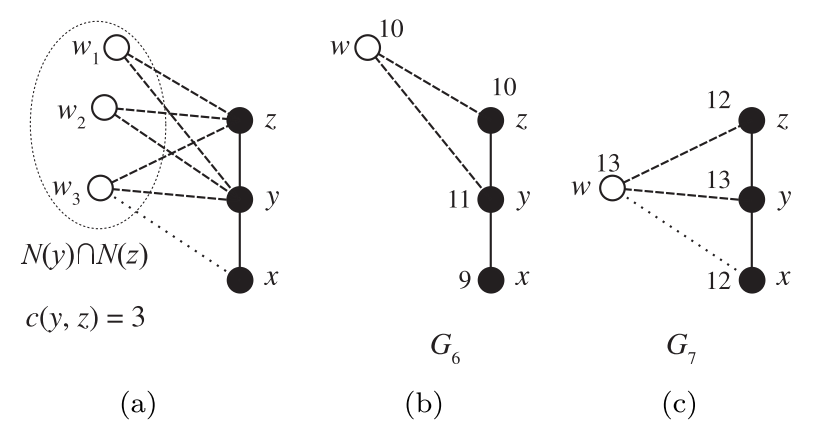
\includegraphics[scale=0.3]{./4-node-graphlet-1.png}
\caption{رابطه بین اوربیت‌های $O_9$ و $O_{12}$.}
\label{fig:o9-o12-relation}
\end{figure}

\begin{figure}[b]
\centering
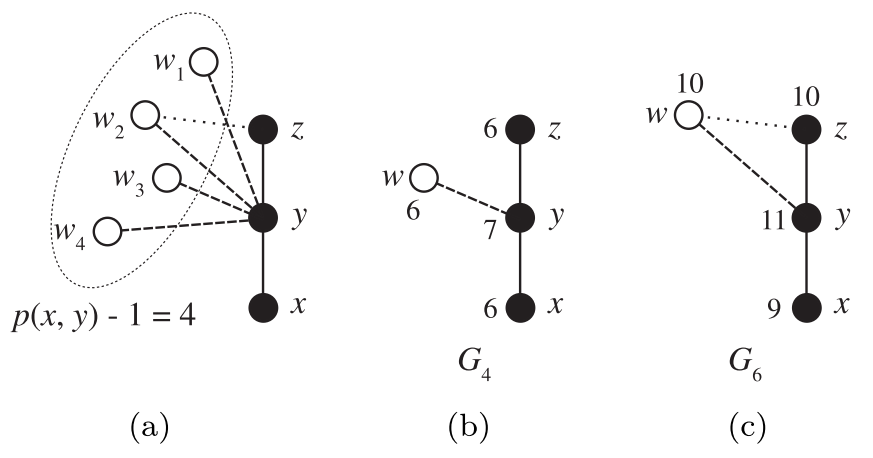
\includegraphics[scale=0.3]{./4-node-graphlet-2.png}
\caption{رابطه بین اوربیت‌های $O_6$ و $O_9$.}
\label{fig:svm-margin}
\end{figure}

حال که تعداد اوربیت $O_{14}$ را داریم، می‌توانیم در زمان ثابت، معادلات را حل کرده و تعداد اوربیت‌های هر رأس را بدست آوریم. بنابراین کل زمان اجرا برای محاسبه تعداد اوربیت‌های تمام رئوس برابر است با $O(m.d+T_4)$ که $O(T_4) = O(d^3)$ زمان مورد نیاز برای شمارش گرافلت‌های کامل روی چهار رأس است.



\subsubsection{شمارش اوربیت‌های پنج رأسی}
برای شمارش اوربیت‌های چهار رأسی، تمام حالت‌های ممکن جهت گسترش یک گرافلت سه رأسی به گرافلت چهار رأسی را در نظر گرفتیم. اینکار برای گذر از چهار رأس به پنج رأس ممکن نیست زیرا تعداد بسیار زیادی معادله بوجود می‌آید که مستقل نیستند. 

\subsection{تبدیل تعداد اوربیت‌ها به تعداد گرافلت‌ها}

\subsection{مقایسه سرعت اجرا}

\section{گرافلت کرنل گاوسی}
فرض کنید برای دو گراف $G$ و $G^\prime$ ، بردار شمارش گرافلت‌ها، $C_G$ و $C_{G^\prime}$ را در اختیار داریم. حال باید این دو بردار را با یکدیگر مقایسه کرده و فاصله آن‌ها را تعیین کنیم. برای کاهش تأثیر اندازه گراف‌ بر مقایسه و همچنین جلوگیری از تأثیر فراوانی زیاد یک گرافلت بر کل مقایسه، بردارها را به صورت
\begin{equation}
\label{eq:feature-vector}
\hat{C}_G = (-\log(\dfrac{C_G(0)}{\sum _{i=0}^{29} C_G(i)}),...,-\log(\dfrac{C_G(29)}{\sum _{i=0}^{29} C_G(i)}))
\end{equation}
نرمال می‌کنیم. حال می‌توان از هر تابع کرنل دلخواهی برای یافتن فاصله این بردارها از یکدیگر، استفاده کرد. طبیعی است که انتخاب تابع مقایسه در دقت کرنل نهایی بسیار تأثیرگذار خواهد بود. همانطور که در بخش \ارجا{sec:compare-kernels-on-graphlet-vector} خواهید دید، تابع گاوسی روی این بردارها بهترین عملکرد را دارد. بنابراین گرافلت کرنل گاوسی $k$ را به صورت
\begin{equation}
\label{eqn:kernelfunction}
k(G,G') = exp(-\gamma\parallel \hat{C}_G - \hat{C}_{G'}\parallel^2)
\end{equation}
تعریف می‌کنیم که در آن $\gamma = \dfrac{1}{2\sigma^2}$ است.

\section{عملکرد گرافلت کرنل گاوسی}
\subsection{داده‌‌ها}
\subsection{شرایط آزمون}
\subsection{گرافلت یا اوربیت؟}\label{sec:graphlet-vs-orbit}
\subsection{میزان دقت در تشخیص مدل‌های تصادفی گراف}

\section{گرافلت کرنل گاوسی روی رئوس}
\section{عملکرد گرافلت کرنل گاوسی روی رئوس}
\subsection{داده‌ها}
\subsection{شرایط آزمون}
\subsection{نتایج}

\section{جمع‌بندی}